\documentclass[11pt,a4paper,twoside]{report}
    \usepackage{a4wide}
    \usepackage{epsfig}
    \usepackage{amsmath}
    \usepackage{tabu}
    \usepackage{amsfonts}
    \usepackage{latexsym}
    \usepackage[utf8]{inputenc}
    \usepackage{listings}
    \usepackage{color}
    \usepackage{titlesec}    
    \usepackage{enumitem}
    \usepackage[catalan]{babel}
    \usepackage{newunicodechar}
    \usepackage{graphicx}
    \usepackage{subcaption}
    \usepackage{float}
    \usepackage{xcolor}
    \usepackage{pgf, tikz}
    \usepackage{listings}
    
  \setcounter{tocdepth}{4}
  \setcounter{secnumdepth}{4}
    
  \newunicodechar{Ŀ}{\L.}
  \newunicodechar{ŀ}{\l.}
  \definecolor{dkgreen}{rgb}{0,0.6,0}
  \definecolor{gray}{rgb}{0.5,0.5,0.5}
  \definecolor{mauve}{rgb}{0.58,0,0.82}
  
  % \lstset{frame=tb,
  % language=Matlab,
  % aboveskip=3mm,
  % belowskip=3mm,
  % showstringspaces=false,
  % columns=flexible,
  % basicstyle={\small\ttfamily},
  % numbers=none,
  % numberstyle=\tiny\color{gray},
  % keywordstyle=\color{blue},
  % commentstyle=\color{dkgreen},
  % stringstyle=\color{mauve},
  % breaklines=true,
  % breakatwhitespace=true,
  % tabsize=3,
  % extendedchars=true,
  % literate={á}{{\'a}}1 {à}{{\`a}}1 {ã}{{\~a}}1 {é}{{\'e}}1 {è}{{\`e}}1 {í}{{\'i}}1 {ï}{{\"i}}1 {ó}{{\'o}}1 {ò}{{\`o}}1 {ú}{{\'u}}1 {ü}{{\"u}}1 {ç}{{\c{c}}}1
  %             {Á}{{\'A}}1 {À}{{\`A}}1 {Ã}{{\~A}}1 {É}{{\'E}}1 {È}{{\`E}}1 {Í}{{\'I}}1 {Ï}{{\"I}}1 {Ó}{{\'O}}1 {Ò}{{\`O}}1 {Ú}{{\'U}}1 {Ü}{{\"U}}1 {Ç}{{\c{C}}}1
  % }
  
  \usepackage{hyperref}
  \hypersetup{
    colorlinks=false, %set true if you want colored links
    linktoc=all,     %set to all if you want both sections and subsections linked
    linkcolor=blue,  %choose some color if you want links to stand out
  }
  
  \setlength{\footskip}{50pt}
  \setlength{\parindent}{0cm} \setlength{\oddsidemargin}{-0.5cm} \setlength{\evensidemargin}{-0.5cm}
  \setlength{\textwidth}{17cm} \setlength{\textheight}{23cm} \setlength{\topmargin}{-1.5cm} \addtolength{\parskip}{2ex}
  \setlength{\headsep}{1.5cm}
  
  \renewcommand{\contentsname}{Continguts}
  \setcounter{chapter}{0}
  % \titleformat{\chapter}[display]
  % {\normalfont\bfseries}{}{0pt}{\Large}
  \titleformat{\chapter}[block]
  {\normalfont\LARGE\bfseries}{\thechapter.}{1em}{\LARGE}
  \titleformat{\section}[block]
  {\normalfont\Large\bfseries}{\thesection.}{1em}{\Large}
  
  \begin{document}
  \tableofcontents
  
  \chapter{Introducció, motivacions, propòsit i objectius}
  
  % \section{Introducció}
  % \section{Motivacions}
  % \section{Propòsit}
  % \section{Objectius}

  La confecció d'horaris de institut es un problema que amaga una alta combinatòria, dificultant-ne molt la seva elaboració manual posat que s'han de prendre moltíssimes decisions a cegues, 
  fent que sigui molt probable cometre errors en la confecció. El HSTT (High School Time Table) consisteix en la solució de forma automàtica de aquest problema d'alta complexitat (NP). 
  Així doncs el problema consisteix en la configuració automàtica de horaris de institut partint de una sèrie de recursos 
  (per exemple: aules, professors, assignatures, grups) i repartir-los de manera que sigui viable i tenint en compte 
  de manera total o parcial les preferències del professorat en quant a horaris, continuïtat, grups, etc. Tot aixó fa que el problema sigui molt difícil de resoldre, degut al gran nombre de combinacions possibles entre els diferents recursos.
  
  Afegint dificultat al problema, depenguen del país del qual estiguem parlant existeixen una gran diversitat de requisits propis, degut a les característiques pròpies del sistema d'estudis secundaris de cada lloc.
  
  Els objectius d'aquest treball són aprofundir en el problema treballat, l'estat actual d'aquest, estudiar les tècniques més utilitzades per resoldre'l actualment. També es pretén solucionar-lo usant les eines desenvolupades recentment pel grup de recerca de Lògica i Programació. Així s'implementarà un generador 
  d'horaris capaç de resoldre el problema utilitzant aquestes tècniques basades en SMT i SAT.
  
  \section{Grup de recerca Lògica i Programació}
  Aquest treball s'emmarca dins del grup de recerca de Lògica i Programació de l'àmbit d'àrea tècnica de la Universitat de Girona.

  El grup basa la seva recerca en l'estudi de satisfactibilitat de formules proposicionals booleanes (SAT) i Satisfiability Modulo Theories (SMT) i les seves
  aplicació per a la resolució de problemes combinatoris com ara problemes de \textit{scheduling} i \textit{planning} arribant a utilitzar amb èxit tècniques innovadores en altres àmbits com
  pot ser: els problemes de \textit{scheduling} i \textit{planning}.

  Durant la elaboració del treball he rebut ajuda i assessorament dels membres del grup, incloent el meu tutor de projecte, el Dr. Josep Suy, qui també en forma part.

%   La introducció serveix per situar el marc del projecte. Aquesta primera etapa implica
% establir les raons que justificaven el desenvolupament del projecte i el que se
% n’esperava obtenir. Aquest propòsit és, per naturalesa, una idea molt ampla.
% Pel contrari, els objectius identifiquen les fites específiques que l’estudiant esperava
% assolir en el seu camí cap al propòsit últim del projecte. Els objectius són més
% precisos que el propòsit general. A partir d’aquesta informació s’ha de comprendre
% millor el projecte, identificar l’entorn on es desenvolupa i entendre millor quina és la
% feina que ha calgut fer.
% En l’apartat anterior, cal precisar i no confondre entre el que són els objectius del
% projecte i els requisits del producte final (aplicació, sistema de maquinari,
% algorismes...).
% En cas que el projecte es desenvolupi en un entorn consolidat (grup de recerca,
% empresa, institució...), aquest apartat pot incloure una descripció de l’entorn en el
% qual es desenvolupa el projecte, així com una especificació del punt de partida del
% projecte. També cal deixar clar en aquest punt quina és l’aportació del P/TFC en
% relació amb el punt de partida.
% En aquest apartat l’estudiant també ha de justificar els apartats de la memòria
% afegits, suprimits o canviats d’ordre respecte del que descriu aquest document.
  \chapter{Estudi de viabilitat}

  % preguntar suy
  %==================
  % Cal justificar quins són els paràmetres que feien possible el desenvolupament del
  % projecte. Aquest punt pot incloure els recursos necessaris per desenvolupar el
  % projecte, els pressupostos inicials, la viabilitat tecnològica i/o econòmica, els
  % recursos humans, etc.
  %

  \chapter{Metodologia i Planificació}
  \section{Metodologia}
  La part més important i grossa d'aquest treball és la creació d'un generador automàtic d'horaris utilitzant les eines oferides per el grup de recerca. 
  Primer caldrà estudiar el problema (HSTT) i la seva duresa, per poder ser capaç d'entendre el què estem treballant.
  Des de aquí es procedirà a la implementació del programa, utilitzant la API SMT creada per el Dr. Jordi Coll, el qual es membre del departament de recerca.
  Aquesta API ens estalviarà la codificació de les restriccions de cardinalitat i les restriccions pseudo-booleanes, 
  apart de oferir-nos una interfície senzilla per poder implementar el model en diferents encodings i múltiples opcions.

  %1 - estudiar el problema
  %2 - fer el parser
  %3 - testejar el parser
  %4 - estudi yices
  %5 - estudi api smt jordi coll
  %6 - fer model
  %7 - testing model
  %8 - proves diferents encodings de les cardinality constraints
  %9 - millora format output
  %10 - si cal, confeccio model
  \section{Planificació}

  Com s'ha dit en l'apartat anterior primer caldrà estudiar el problema HSTT i la seva duresa. 
  Després es procedirà amb el disseny i la implementació del generador. Primer caldrà dissenyar implementar i testejar un \textit{parser} pels fitxers. En aquest pas també cal pensar i implementar en quina estructura es guardaràn aquestes dades i com es transferiràn en el model que es codificarà posteriorment. 

  Al tenir el \textit{parser} i l'estructura de dades enllestits caldrà començar a estudiar com funciona la API per C++ del yices i 
  posteriorment la API SMT del Dr. Jordi Coll. Això ens permetrà començar a dissenyar, codificar i testejar el model, que és el següent pas del treball. 
  Al tenir enllestit el model, es faràn les proves de rendiment amb diferents límits de optimització i diferents encodings de les restriccions de cardinalitat.
  Finalment s'implementarà una forma maca i llegible de mostrar els horaris generats.
  
  Amb això el generador es donarà per acabat i es passarà a la confecció de la memòria del treball. 

  %%diagrama de gent...




  \chapter{Marc de treball i conceptes previs}
  \section{Definició del problema}
  \section{Format XHSTT}
  \section{Cardinality encodings}
  \section{Estat de l'art}
  





  \chapter{Requisits del sistema}

  En aquest treball es pretén desenvolupar un programa en C++ que haurà de ser capaç de rebre un fitxer xml en format XHSTT, llegir-lo, codificar-ne el model a yices, resoldre'l i mostrar-ne el resultat de forma llegible. 
  Per fer això requerirem d'una llibreria que ens permeti llegir fitxers XML (en aquest cas s'ha decidit utilitzar pugixml\footnote{https://pugixml.org/}). També requerirem insta\l.lar el yices\footnote{https://yices.csl.sri.com/}. 
  Posat que la API SMT del Dr. Jordi Coll està desenvolupada per a linux, necessitarem que la màquina on s'executi utilitzi de sistema operatiu una distribució de Linux amb un compilador C++. 
 % TODO: CAL COMPLETAR!!
 

  \chapter{Estudis i decisions}
  \section{Programari utilitzat}

  A continuació s'enumera tot el programari que s'ha utilitzat per la confecció d'aquest treball:
  \begin{itemize}
  \item El solver utilitzat és el Yices versió 2.6.1 degut a que és dels millors que hi ha i el grup de recerca hi te experiència prèvia. 
  \item Per la lectura de les instancies XHSTT s'ha utilitzat la llibreria pugixml versió 1.9-1. S'ha decidit usar aquesta llibreria pel fet de que ja hi tenia experiència prèvia.
  \item La codificació del generador s'ha fet en C++ 17 i s'ha compilat amb el gcc versió 9.1.0-2 perqué és amb el que es treballa al departament i permet la utilització de la API SMT del Dr. Jordi Coll. Per desenvolupar s'ha utilitzat el IDE qtCreator 4.9.2-3.
  \item La elaboració d'aquesta memòria s'ha fet amb \LaTeX, utilitzant com a IDE el Microsoft Visual Studio Code amb la versió lliure per linux 1.37.1-1, juntament amb l'expansió LaTeX Workshop (versió 5.6.0). 
  \end{itemize}

  \section{Maquinari utilitzat}
  Per efectuar les proves de rendiment s'ha utilitzat un ordinador amb les següents especificacions:
  \begin{itemize}
    \item Processador AMD Ryzen\textsuperscript{TM} 3 1200 a 3.5 GHz amb 4 nuclis físics,  10MB de memòria cau i arquitectura 64 bits.
    \item 16GB de memòria RAM DDR4 a 3333MT.
    \item Sistema operatiu Arch Linux 64 bits amb kernel Linux 5.2.9.arch1-1
  \end{itemize} 


  \chapter{Anàlisis i disseny del sistema}

  \section{Anàlisis}
  % En la fase d’anàlisi cal detallar el model de dades i el model de processos. 
  \subsection{Necessitats del sistema}
  Les necessitats principals del sistema són les següents: 
  \begin{itemize}
    \item Necessitem rebre un fitxer de l'usuari.
    \item Necessitem llegir les dades de un fitxer XHSTT tal i com s'ha explicat anteriorment, per tant requerirem de un \textit{parser} per ferho.
    \item Necessitarem guardar les dades i les restriccions de alguna manera.
    \item Necessitarem un model lògic i codificar-lo utilitzant la API SMT del Dr. Jordi Coll. 
    \item Necessitarem processar i guardar les dades de manera que ens faciliti el mostrar-les de forma que es pugui entendre.
    \item Necessitarem comprovar en la mesura del possible que la instància XHSTT sigui correcta.
  \end{itemize}

  \subsection{Anàlisis de processos}
  Pel que fa els processos no serà gaire complicat. L'usuari cridarà el programa, el programa s'encarregarà de codificar el model pel yices i cridar-lo per resoldre'l, utilitzant la llibreria per C++ pròpia del yices.


  
  \section{Disseny}    
  % En la fase de disseny cal determinar les interfícies d’usuaris, els models físics de 
  % dades, (no cal)els models físics de processos i, si escau, el model d’objectes. En aquest 
  % àmbit, els patrons de disseny permeten reutilitzar solucions generals a problemes 
  \section{Interfícies d'usuari}
  El programa funcionarà via consola. Les dades necessàries, com ara el fitxer amb la instància, es passaran per paràmetres, utilitzant el sistema existent en la API SMT del Dr. Jordi Coll.
  \section{Model de dades}

  El model de dades correspondria al següent diagrama:
  \begin{figure}[h!]
    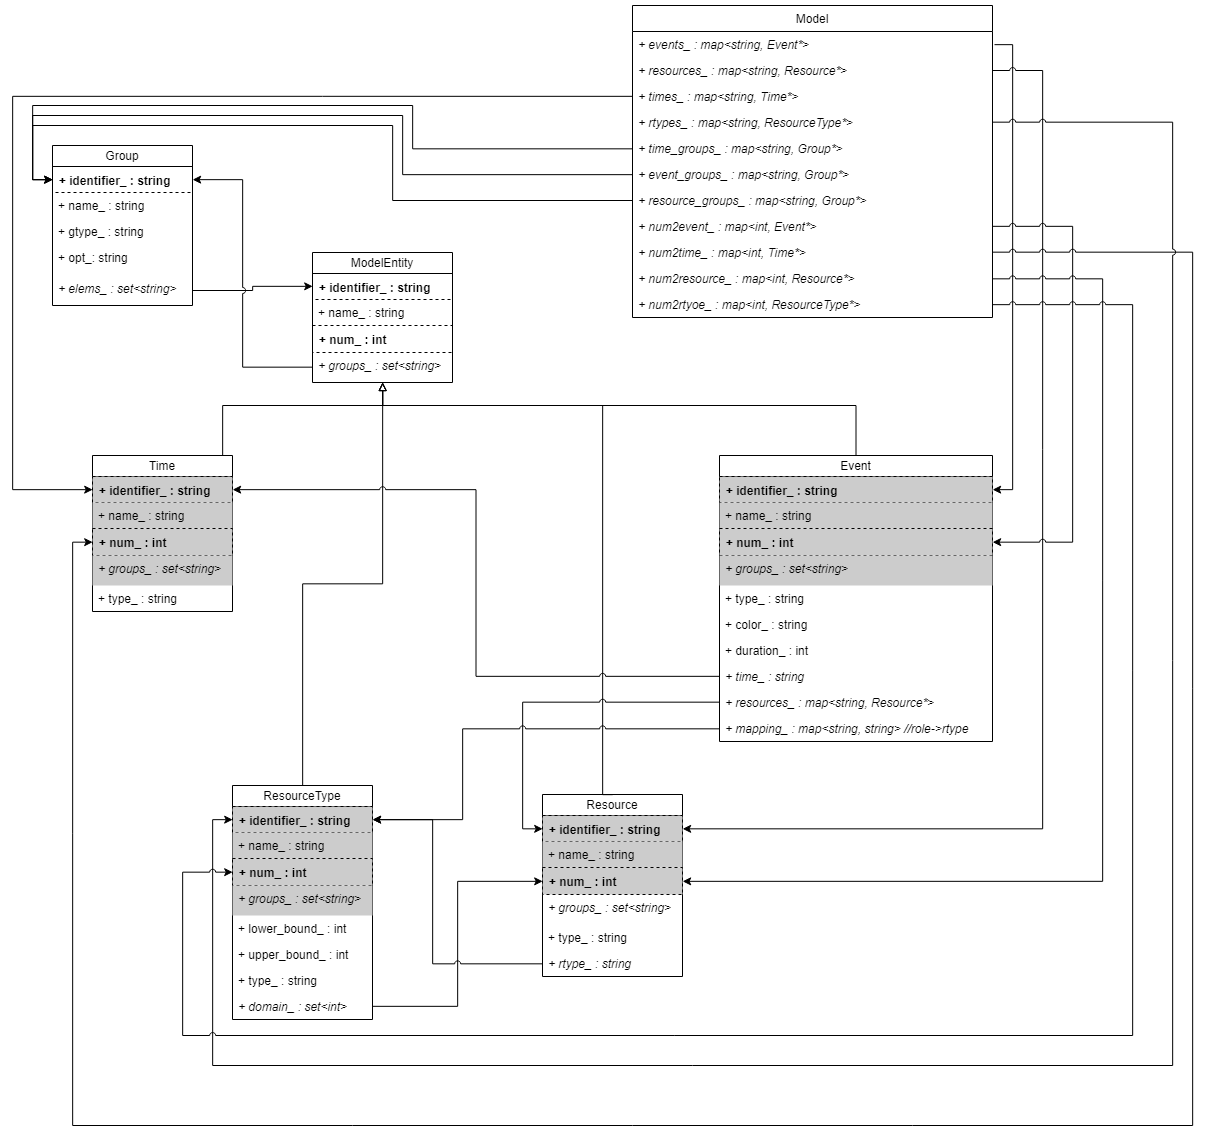
\includegraphics[width=\textwidth]{Diagrames/ModelDades.png}
    \caption{Model de Dades}
    \label{fig:DataModel}
  \end{figure}

  \section{Model d'objectes}

  El model d'objectes correspondria al següent diagrama:
  \begin{figure}[h!]
    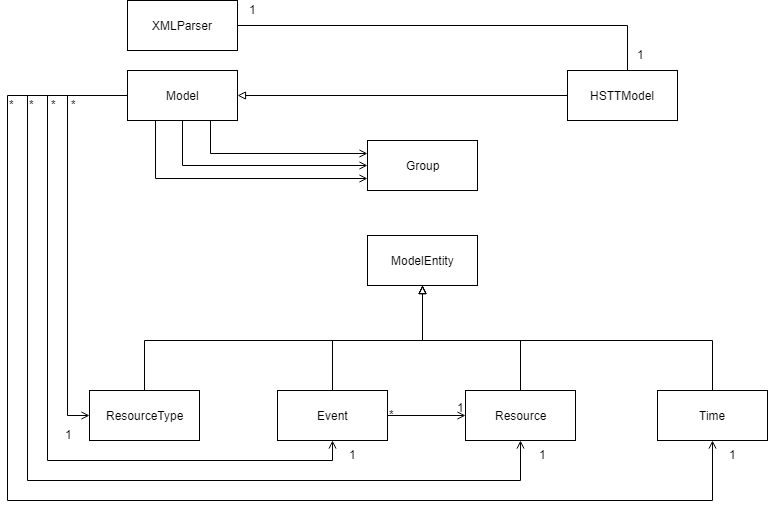
\includegraphics[width=\textwidth]{Diagrames/UMLKai.png}
    \caption{Model d'objectes}
    \label{fig:ObjectModel}
  \end{figure}
  



  

  \chapter{Implementació i proves}
   
  % En aquest apartat es detallen els problemes i les solucions apareguts en la 
  % implementació, així com, si és el cas, el model de classes i els algorismes més 
  % rellevants. 
  
  % A més, cal detallar les proves, tant unitàries com de sistema, que es realitzen. 
    
  \chapter{Implantació i resultats}
  % Aquest apartat ha de descriure amb detall el procés de desenvolupament que ha 
  % calgut dur a terme per implantar el sistema desenvolupat. L’apartat de resultats ha 
  % de mostrar clarament el grau d’assoliment dels objectius, mitjançant exemples del 
  % funcionament d’allò que s’ha fet. 
   
  % Es revisarà i valorarà que el sistema desenvolupat compleixi amb la legislació i 
  % normatives vigents, especialment en el que fa referència a la llei orgànica de 
  % protecció de dades de caràcter personal (LOPD) i a la llei de serveis de la societat 
  % de la informació i comerç electrònic (LSSICE). 
   
  % A més, ha de mostrar que l’aplicació resultant del projecte fa les tasques 

  \chapter{Conclusions}
  \chapter{Treball futur}
  \chapter{Bibliografia}
  \chapter{Manual d'usuari i insta\l.lació}
  
  
  \end{document}
  